
\chapter{Arquitetura de Software}
\label{sec-arquitetura}

A arquitetura de software do sistema~\imprimirtitulo \,\,segue a arquitetura padrão sugerida pelo FrameWeb~\cite{souza:masterthesis07,souza-et-al:iism09} baseada no padrão Camada de Serviço~\cite{fowler:book02}. A Figura~\ref{figura-arquitetura-padrao} ilustra a arquitetura estabelecida pelo método FrameWeb.

\begin{figure}[h]
	\centering
	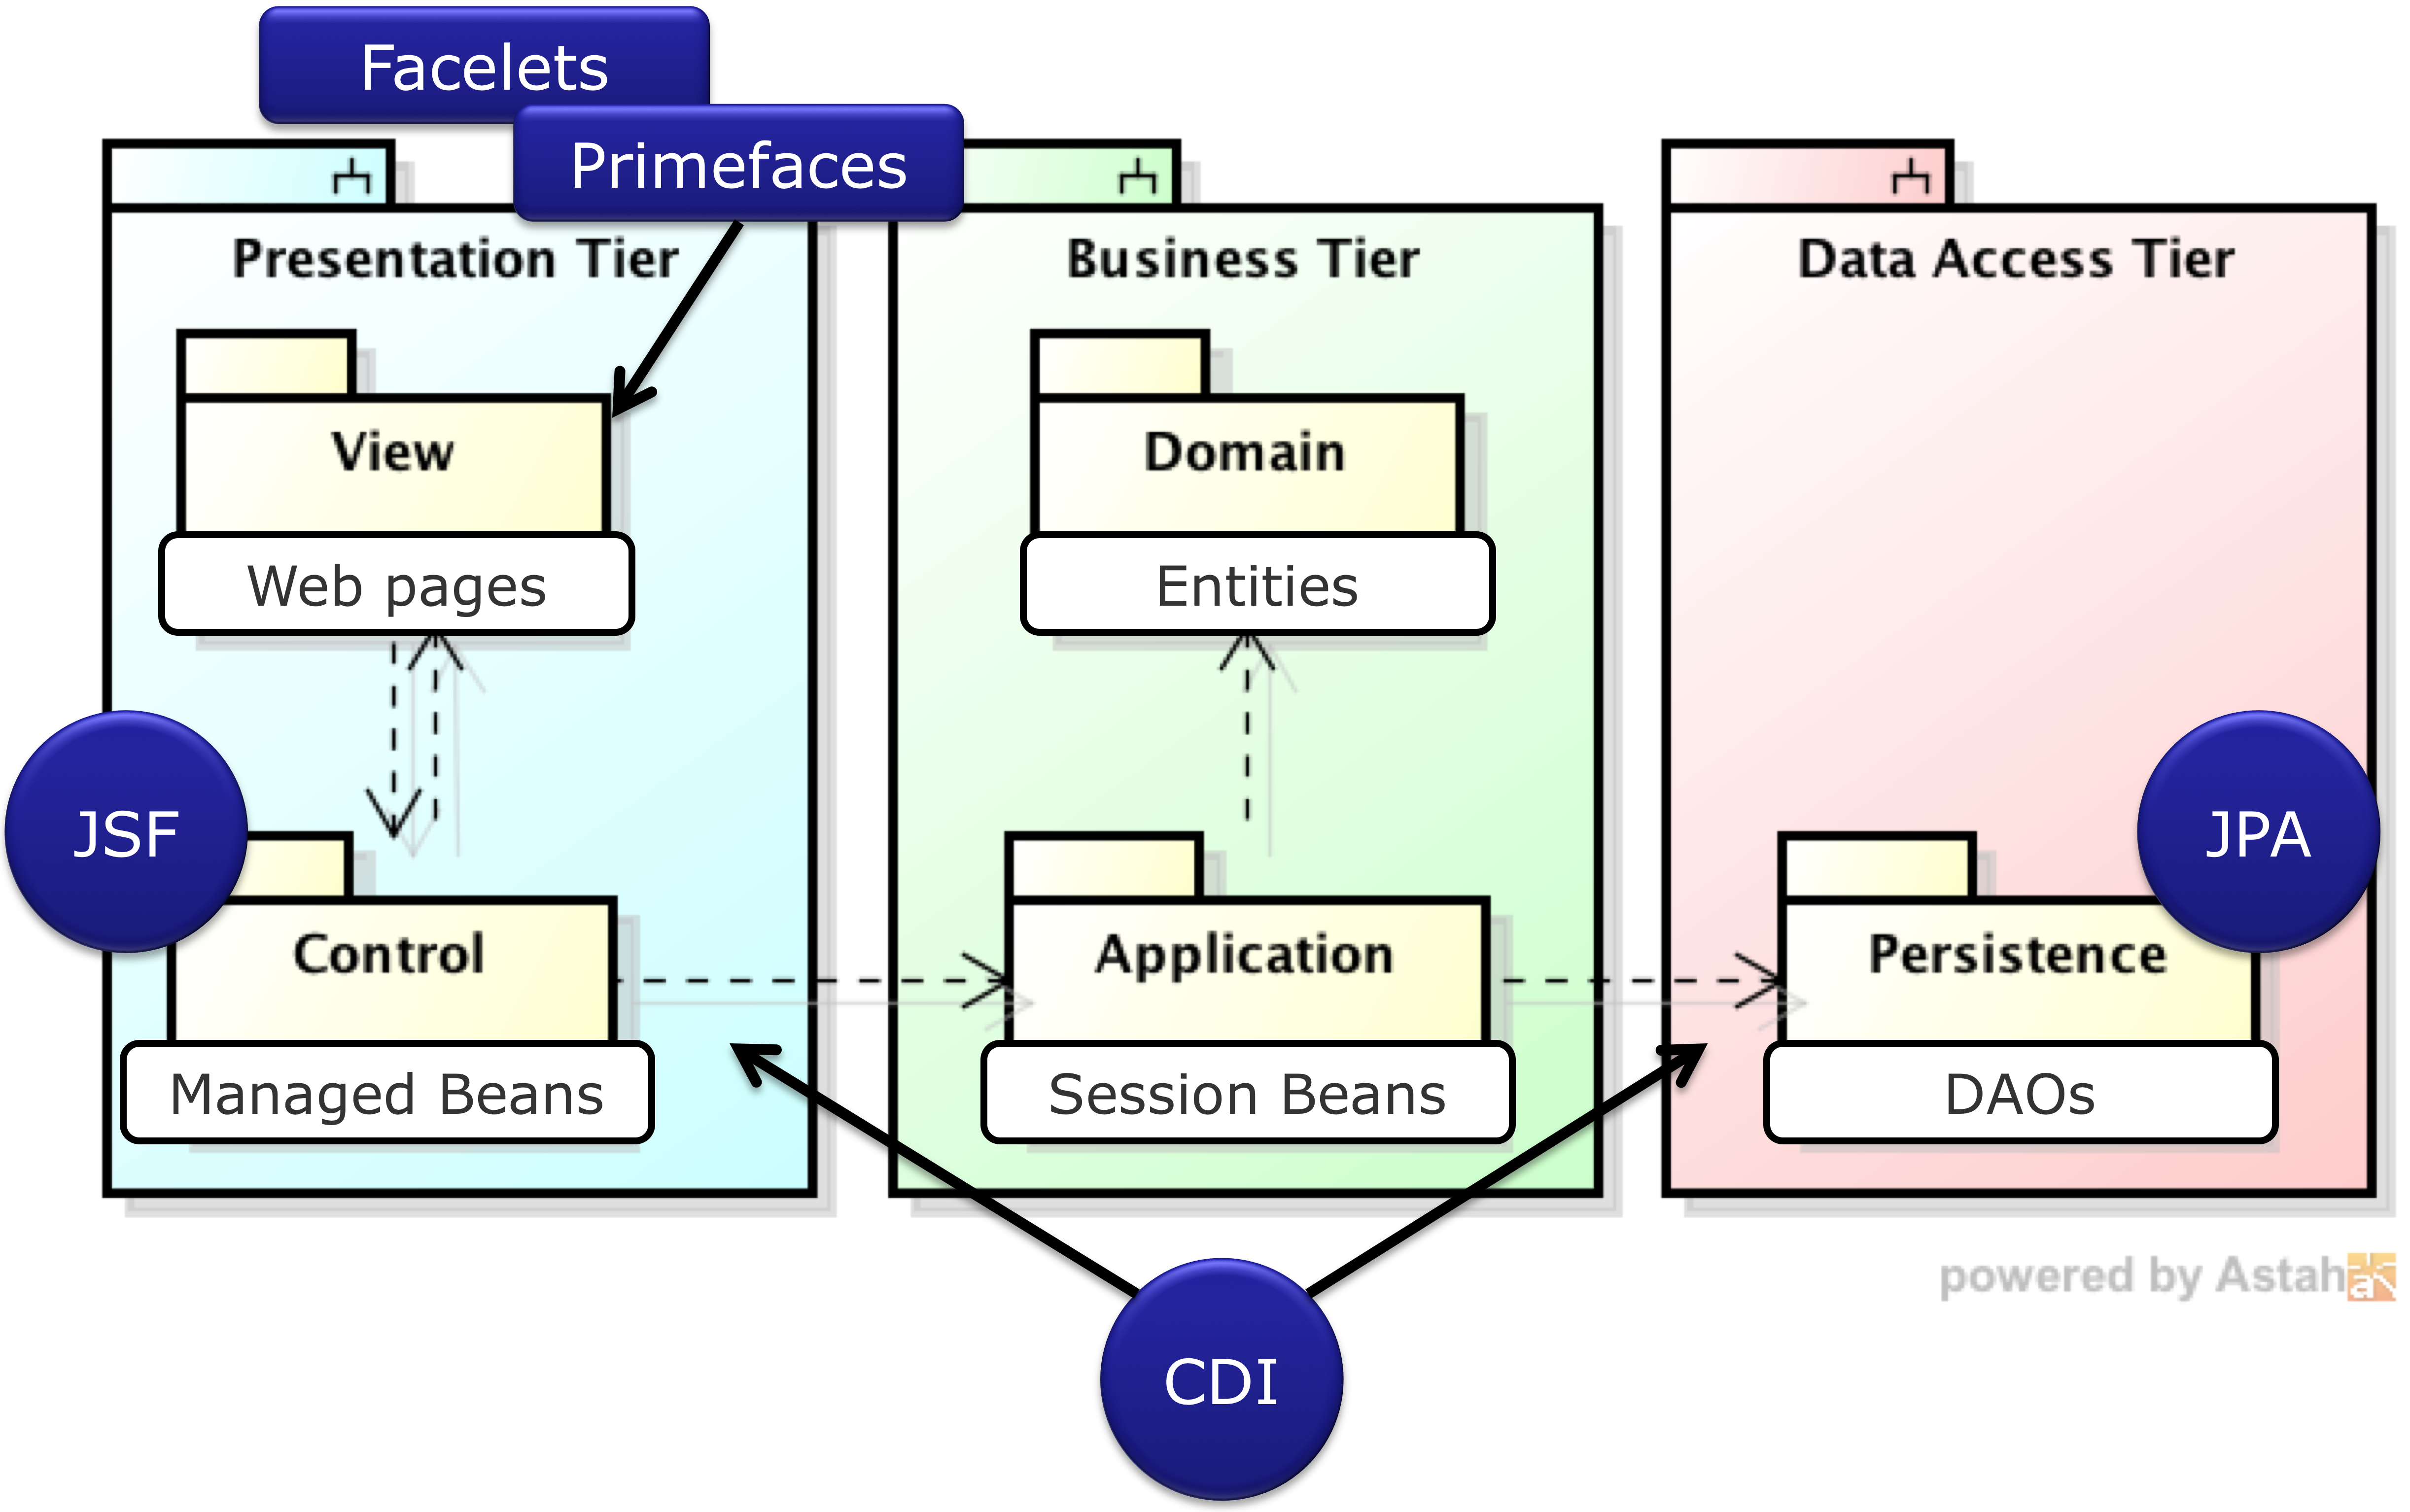
\includegraphics[width=0.9\textwidth]{figuras/figura-arquitetura-padrao.png}
	\caption{Arquitetura padrão proposta pelo FrameWeb.}
	\label{figura-arquitetura-padrao}
\end{figure}

Nas próximas seções, serão apresentados diagramas FrameWeb relativos a cada uma das camadas da arquitetura do sistema.


\section{Camada de Apresentação}
\label{sec-arquitetura-apresentacao}

%\vitor{Apresentar os modelos de navegação do FrameWeb.}

Possui a responsabilidade de realizar a interação entre o sistema e o usuário, exibindo as informações e interpretando os comandos em ações da persistência de dados e da lógica de negócio. Apresenta os modelos de navegação, que auxiliam os desenvolvedores na implementação dos componentes e das classes dos pacotes Visão e Controle.

Um Modelo de Navegação foi gerado para cada caso de uso neste projeto, no entanto, alguns casos de uso não foram apresentados, pois possuem o mesmo modelo de navegação apresentado na Figura \ref{figura-arquitetura-navegacao1}. Os casos de uso que foram omitidos foram: Cadastrar Chefe do Departamento, Solicitar Afastamento, Manifestar-se Contra Afastamento, Encaminhar Afastamento e Registrar Parecer Relator.  

\begin{figure}[h]
	\centering
	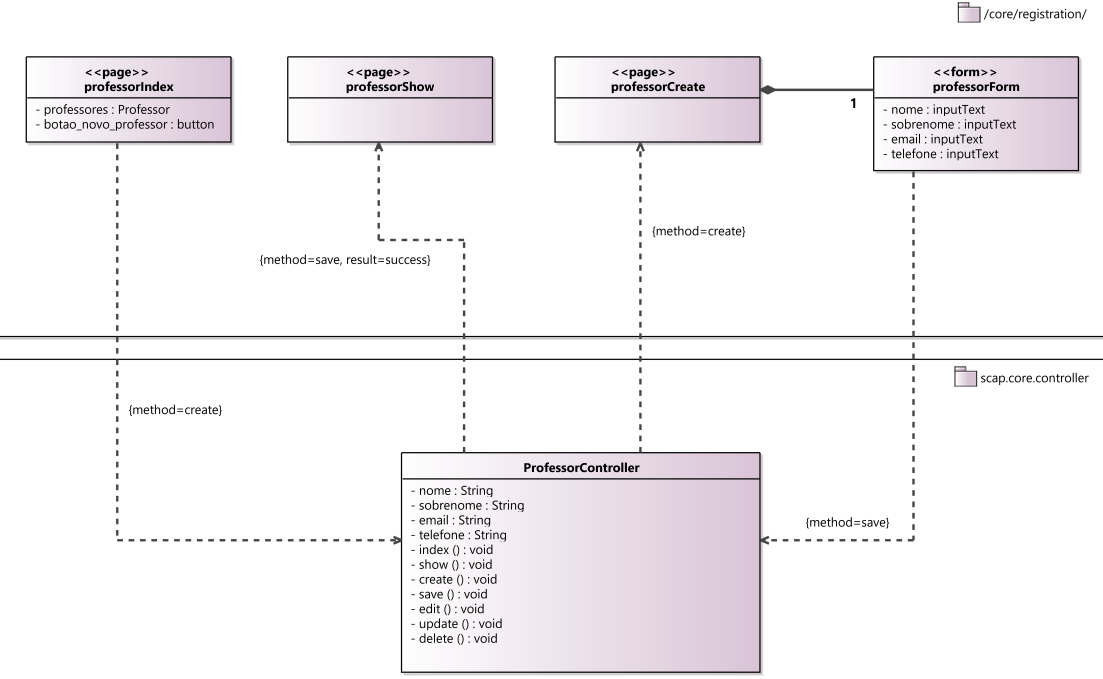
\includegraphics[width=1\textwidth]{figuras/figura-arquitetura-navegacao1.png}
	\caption{Modelo de Navegação do Caso de Uso: Cadastrar Usuário (Professor).}
	\label{figura-arquitetura-navegacao1}
\end{figure}

De mesmo modo, outros casos de uso também não foram apresentados por seguirem o mesmo modelo de navegação representado pela Figura \ref{figura-arquitetura-navegacao2}. Assim, ficaram omitidos os casos de uso: Registrar Parecer CT, Registrar Parecer PRPPG e Cancelar Afastamento. 

\begin{figure}[h]
	\centering
	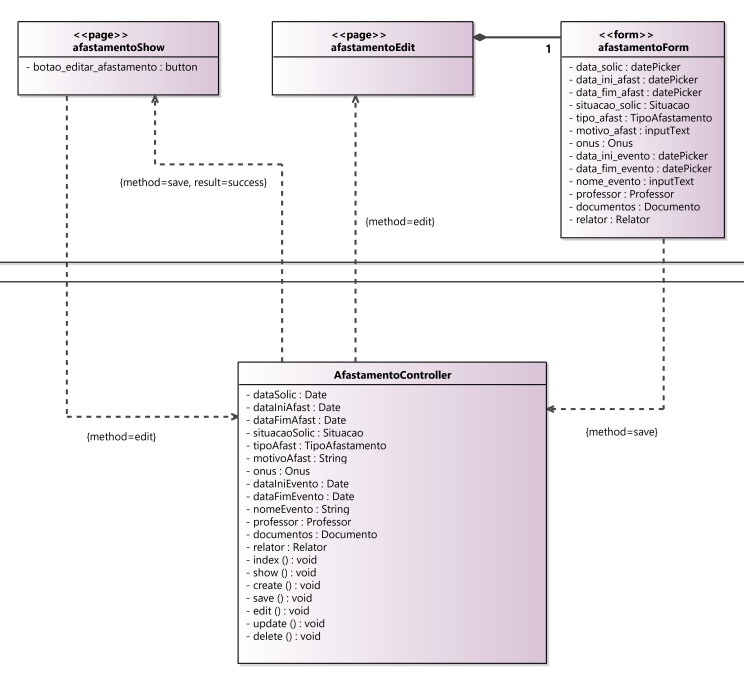
\includegraphics[width=1\textwidth]{figuras/figura-arquitetura-navegacao2.png}
	\caption{Modelo de Navegação do Caso de Uso: Arquivar Afastamento.}
	\label{figura-arquitetura-navegacao2}
\end{figure}

\section{Camada de Negócio}
\label{sec-arquitetura-negocio}

%\vitor{Apresentar os modelos de entidades e de aplicação do FrameWeb.}

Engloba as funcionalidades que dão suporte aos processos de negócio, concentrando as regras de negócio, conceitos do domínio, cálculos e processamentos. Representado por um diagrama de classes da UML, o Modelo de Domínio apresenta o mapeamento dos objetos de domínio do problema para a persistência em banco de dados relacional. Esse modelo pode ser visualizado na Figura \ref{figura-arquitetura-entidade} e na Figura \ref{figura-arquitetura-enum}.  

\begin{figure}[h]
	\centering
	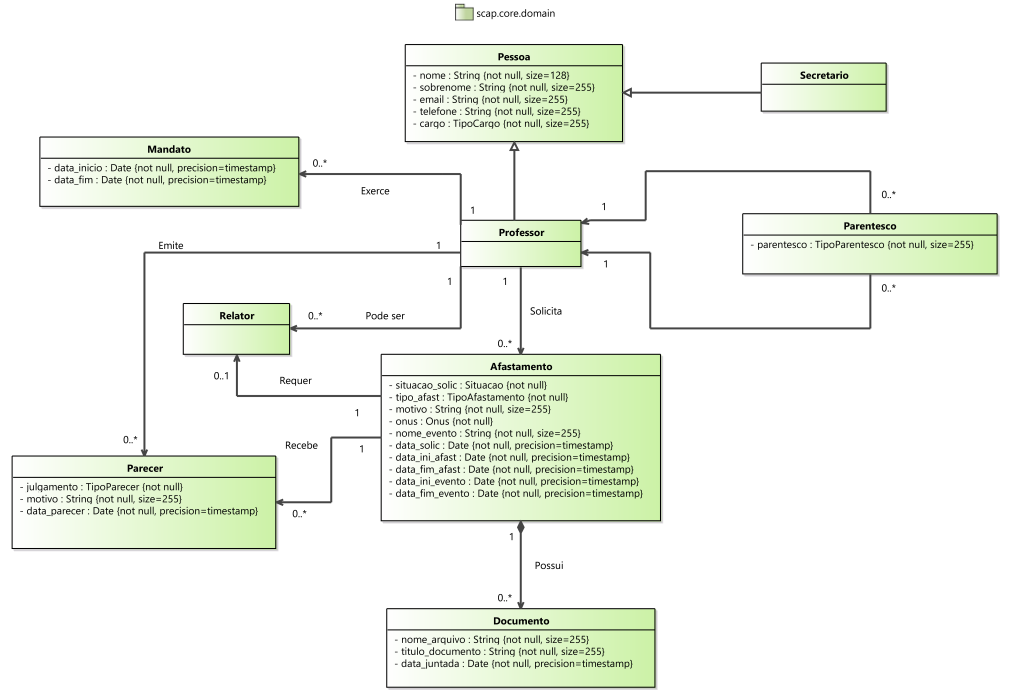
\includegraphics[width=1\textwidth]{figuras/figura-arquitetura-entidade.png}
	\caption{Modelo de Entidades.}
	\label{figura-arquitetura-entidade}
\end{figure}

\begin{figure}[h]
	\centering
	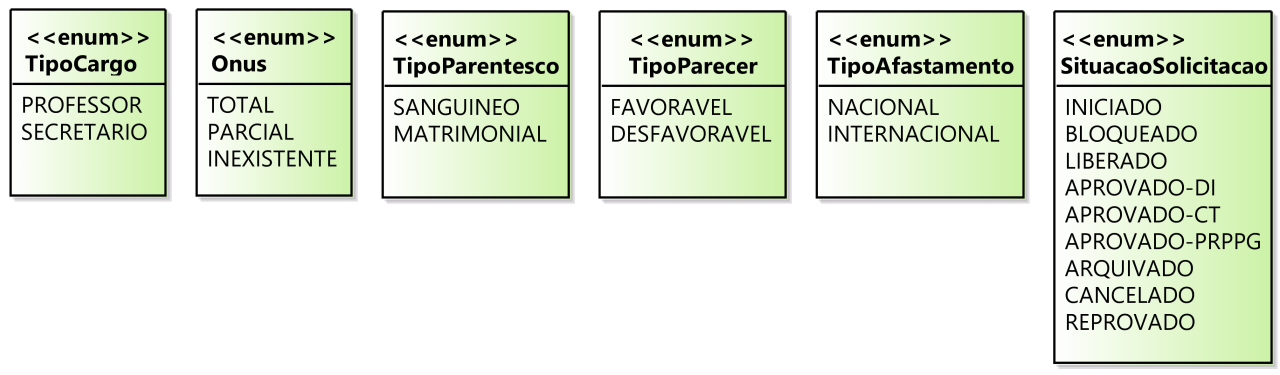
\includegraphics[width=1\textwidth]{figuras/figura-arquitetura-enum.png}
	\caption{Tipos Enumerados do SCAP.}
	\label{figura-arquitetura-enum}
\end{figure}

O diagrama do Modelo de Aplicação é utilizado para auxiliar os desenvolvedores na implementação das classes do pacote Aplicação e na configuração das dependências entre os pacotes Controle, Aplicação e Persistência. Neste projeto foram gerados um modelo de aplicação para cada \textit{Data Access Object} (DAO) existente. Portanto, por seguirem o mesmo padrão, foram representados apenas dois modelos de aplicação que podem ser visualizados na Figura \ref{figura-arquitetura-aplicacao}. 

\begin{figure}[h]
	\centering
	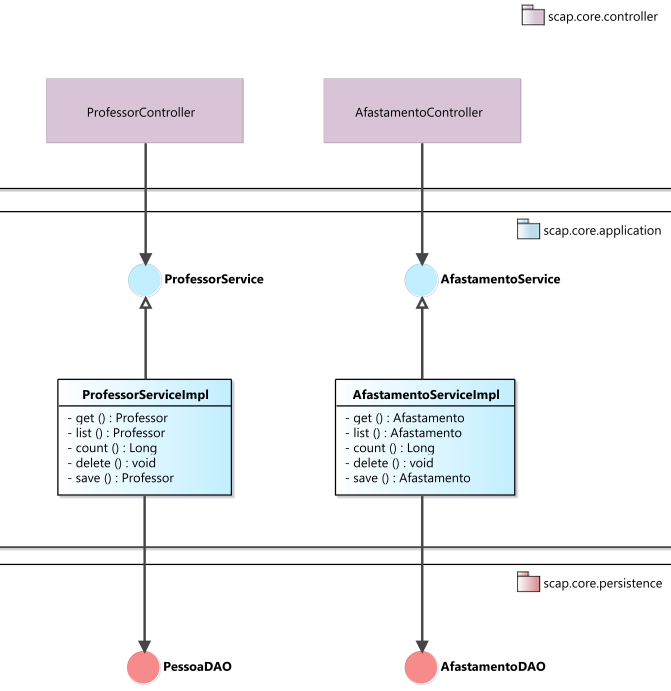
\includegraphics[width=1\textwidth]{figuras/figura-arquitetura-aplicacao.png}
	\caption{Modelo de Aplicação.}
	\label{figura-arquitetura-aplicacao}
\end{figure}

\section{Camada de Acesso a Dados}
\label{sec-arquitetura-dados}

%\vitor{Apresentar os modelos de persistência do FrameWeb.}

Estabelece o acesso a dados, gerenciando requisições e cuidando da sincronização de elementos de dados. Um diagrama de classes da UML representa as classes DAO existentes, que são responsáveis pela persistência das instância das classes de domínio. Esse diagrama pode ser visualizado na Figura \ref{figura-arquitetura-persistencia}.

\begin{figure}[h]
	\centering
	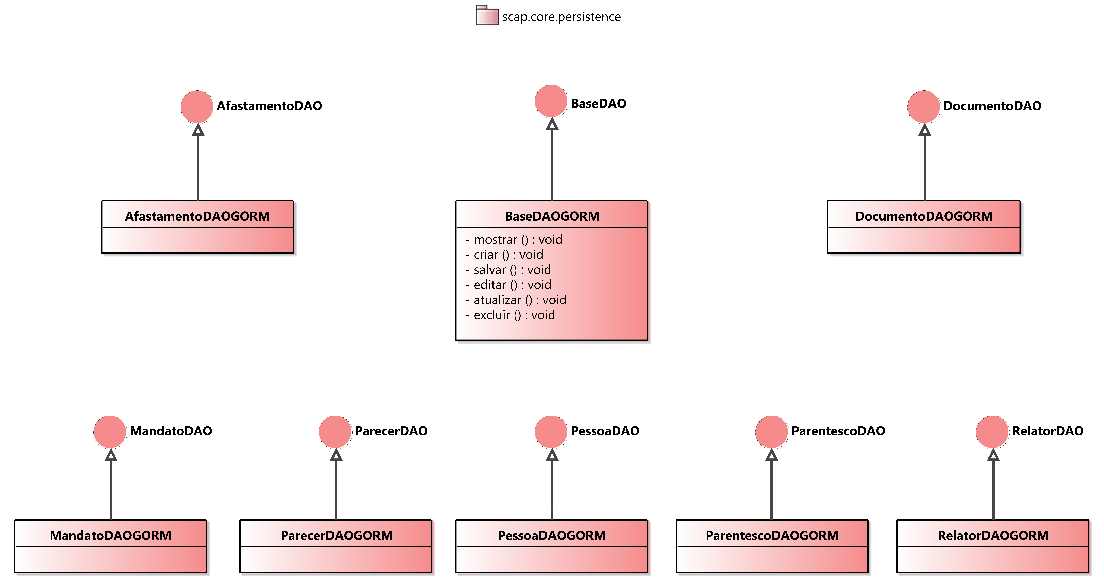
\includegraphics[width=1\textwidth]{figuras/figura-arquitetura-persistencia.png}
	\caption{Modelo de Persistência.}
	\label{figura-arquitetura-persistencia}
\end{figure}

